\documentclass{llncs}
%%%%%%%%%%%%%%%%%%%%%%
%%%%   PACKAGES   %%%%
%%%%%%%%%%%%%%%%%%%%%%
\usepackage{makeidx}
\usepackage{amsmath}
\usepackage{amssymb}
\usepackage{stmaryrd}
\usepackage{graphicx}
\usepackage{subfigure}
\usepackage{latexsym}
\usepackage{url}
\usepackage{color}
\usepackage{isabelle}
\usepackage{isabellesym}
\usepackage{theorem}
\usepackage{multicol}
\usepackage{algorithmic}
\usepackage[linesnumbered,ruled,vlined]{algorithm2e}
\usepackage{multicol}
\usepackage{enumitem}
%%%%%%%%%%%%%%%%%%%%%%%%%%%%
%For Isabelle code
\newlength{\fminilength}
\newsavebox{\fminibox}
\newenvironment{fmini}[1][\linewidth]
  {\setlength{\fminilength}{#1\fboxsep-2\fboxrule}%
   \vspace{2ex}\noindent\begin{lrbox}{\fminibox}\begin{minipage}{\fminilength}%
   \mbox{ }\hfill\vspace{-2.5ex}}%
  {\end{minipage}\end{lrbox}\vspace{1ex}\hspace{0ex}%
   \framebox{\usebox{\fminibox}}}

\newenvironment{specification}
{\noindent\scriptsize
\tt\begin{fmini}\begin{tabbing}X\=X12345\=XXXX\=XXXX\=XXXX\=XXXX\=XXXX
\=\+\kill} {\end{tabbing}\normalfont\end{fmini}}
\def \twoSpaces {\ \ }
%%%%%%%%%%%%%%%%%%%%%%%%%%%%

%%%%%%%%%%%%%%%%%%%%%%%%%%%%
%for comments
\newcommand\JP[1]{\textcolor{magenta}{JP: #1}}
\newcommand\lyj[1]{\textcolor{green}{lyj: #1}}

\newcommand{\bedt}[1]{{\color{black}#1}}
\newcommand{\forget}[1]{}

\def \pInv {i}

\def \twoSpaces {\ \ }
\def \oneSpace {\ }
\def \eqc {\doteq }
\def \andc {\barwedge }
\def \negc {!}
\def \orc {\veebar }
\def \alt {$/\backslash$ }
\def \cat {\symbol{94}}

\def \dbRight {$\backslash\backslash$}
\def \iInv {iInv}
\def \iR {iR}
%%%%%%%%%%%%%%%%%%%%%%%%%%%%
%\def \pInv1 {i2}
%\def $\wedge$ {$\wedge$}
%\def $\Rightarrow$ {$\Rightarrow$}
%\def  \<equiv> {$\equiv$}
%%%%%%%%%%%%%%%%%%%%%%%%%%%

%%%%%%%%%%%%%%%%%%%%%%%%%%%
% Additional math operators
%%%%%%%%%%%%%%%%%%%%%%%%%%%

\usepackage[colorlinks,
            linkcolor=black,
            anchorcolor=black,
            citecolor=blue,
            urlcolor=black,
            bookmarks=true
            ]{hyperref}

%\input{tcilatex}

%=========================================
\begin{document}

\title{  An Automatic Parameterized Verification of  FLASH Cache Coherence Protocol by Paraverifier}
\titlerunning{paraVerifier: An Invariant Finder}
\author{Yongjian Li \inst{1} \and
        Kaiqiang Duan \inst{1} \and
       % Shaowei Cai \inst{1} \and
        Yi Lv \inst{1} }
\authorrunning{Li et al.}
\institute{
State Key Laboratory of Computer Science,
%Institute of Software,
Chinese Academy of Sciences
}

\maketitle

%-------------------------------------------------------------------------
\begin{abstract}
%-------------------------------------------------------------------------
The FLASH protocol is an industrial-scale cache coherence protocol, whose parameterized verification is a notoriously hard challenge to the field of formal \bedt{verification}. In this paper, we show how to verify its important properties by our tool {\sf paraverifier}. Being distinguished from any other approach, our proof product is a formal  proof with a set of inductive invariants. %by induction in Isabelle and a series of message flows which reflect the semantics of the protocol intuitively.
\bedt{On one hand, both invariants are searched automatically and the formal proof is generated automatically in our work, thus tedious human labor can be obviated. On the other hand, the formal proof guarantees the most rigorous correctness of the parameterized verification. Besides, we make efforts to illustrate the semantic intuition behinds these invariants, thus our proof product is not only a certification of correctness, but also a comprehensive analysis report.}
%Among all the work, our work is the most automatic, and the  set of auxiliary invariants is the most complete. Both invariants are searched automatically and the formal proof is generated automatically. Besides, we make efforts to illustrate the semantic intuition behinds these invariants.
%delay and early versions of FLASH protocol are verified, and the differences between the two versions can be reflected in the auxiliary invariants and flow charts for them found by the tool.

%-------------------------------------------------------------------------
\end{abstract}
%-------------------------------------------------------------------------

%=========================================
\section{Introduction}\label{sec:introduction}
%=========================================
Verification of parameterized concurrent systems is interesting in
the area of formal \bedt{verification}, mainly due to the practical importance
of such systems. Parameterized systems exist in many important
application areas: cache coherence protocols, security systems, and
network communication protocols, \emph{etc}. In this work, we will
focus on a real-world cache coherence protocol - Stanford FLASH protocol \cite{FLASHCache}. The challenge posed by
parameterized verification is that the desired properties should
hold in any instance of the parameterized system. %The core of
%parameterized verification is the construction of a set of auxiliary
%invariants~\cite{Pnueli2001,Chou2004,Pandav2005,cubicle2011}, which
%are either used for inductive verification or abstraction model
%construction. Therefore, how to find these auxiliary invariants is
%the central problem in the research field of parameterized
%verification.
%\JP{It is unclear what is the initial invariant and what are the correctness proofs.}
%\JP{To make the concepts clear, it will be better to briefly describe the standard
%procedure for parameterized verification.
%Then you can talk about initial invariant, correctness proofs, auxiliary invariants, etc.
%(Such terms are not explained so far in the current paper.)}
%\JP{Here, still the statement of the research problem is missing.
%Why an invariant finder is needed (the motivation)?}

FLASH protocol is a publicly-recognized challenging benchmark in the field of formal
 verification. In the pioneering work,
Park and Dill applied the general purpose theorem prover PVS \cite{cade92-pvs}
to   verify the protocol for arbitrary $N$ nodes \cite{Park1996a}. This is a laborious process, since they introduce a simplified  FLASH protocol with the so-called aggregated transactions, which
is, in fact,  an abstracted version of FLASH protocol, and  need to prove
the correspondence between the abstract and the original FLASH
protocol, and then prove the correctness of the abstracted protocol, and subsequently derive the correctness of  the
original protocol by the correspondence. %New   auxiliary state variables like {\tt fwdSrc} are   introduced  for verification. Deep human insight for FLASH protocol is needed for both the construction of the abstracted protocol  and  introducing new state variables.
Inductive invariants are provided by \bedt{hand}, and the theorem prover must be manually guided to perform the induction proof to prove the correspondence between the simplified protocol  and the original one. %This work is really pioneering because later research on FLASH protocol must also rely on the version of FLASH protocol in \cite{}. Especially, the auxiliary
%variables proposed  are reserved and needed for verification in later work.

McMillan applies methods of compositional model
checking \cite{McMillan2001} to the verification of FLASH protocol by using Cadence-SMV \cite{cadenceSMV}. %This approach has the advantage that parameterized
%systems can be proved correct without the need to state inductive invariants explicitly,
%since invariant information is obtained by model checking abstract systems.
Safety and liveness of the
FLASH protocol are both verified. Despite the fact that SMV is designed as a model-checker to  check automatically properties, the core techniques for FLASH protocol parameterized verification adopted by McMillan is SMV's advanced features for proofs such as composition proof and temporal case splitting, and abstraction. Human interaction must be heavily relied on to  guide SMV to work, depending on his insight into FLASH protocol. Unlike a general theorem prover like Isabelle, SMV does not have a good logical foundation and mechanism to perform theorem proving process. Briefly speaking, the above proofs have the cons as follow: lacking of rigorousness as a theorem prover, rough understanding for non-specialists of SMV, as well as the limitation of generalization to other protocol case studies and implementation in general-purpose theorem provers. \forget{The above proofs are neither rigorous as a theorem prover, nor easily understood to a non-specialist of SMV.  Because these proof techniques are  only special for SMV,  they are  difficult to be generalized to other protocols and to be implemented in a general-purpose theorem prover.}

The CMP method, which adopts parameter abstraction and guard strengthening, is proposed
in~\cite{Chou2004} for verifying a safety property $inv$ of
a parameterized system.
 An abstract instance of the parameterized protocol,  which consists of m + 1
nodes $\{P_1, \ldots , P_m, P^*\}$ with $m$ normal nodes plus one
abstract node $P^*$, is constructed iteratively. The abstract system is an
abstraction for any protocol instance whose size is greater than
$m$. Normally the initial abstract system does not satisfy the
invariant $inv$. Nevertheless, it is still submitted to a model
checker for verification. When a counterexample is produced, people need to
carefully analyze it and come up with an auxiliary invariant
$inv'$, then use it to strengthen the guards of some transition
rules of the abstract node. The ``strengthened'' system is then
subject to model checking again. This process stops until the
refined abstract system  eventually satisfies the original invariant
  as well as all the auxiliary invariants supplied by people. %However, this method's soundness is only argued in an informal way. To the best of our knowledge, no one has formally proved its correctness in a theorem prover. This situation may be not ideal because its application domain for cache coherence protocols  which demands the highest assurance for correctness.
\bedt{The CMP method has been extended by \cite{Talupur2008a} that the ``message flow'' can be used as invariants. These ``flow'' invariants is obtained manually by people who carefully analyze the design documents.
 However, the downside of the CMP method is that the analysis of counter-example and generation of new auxiliary invariants usually
 depend on human's deep insightful understanding of the protocol.} It is too laborious for people to do this analysis and some effective automatic  tool is needed.% to help people.

\bedt{In \cite{cubeicBeyond}, an algorithm, called BRAB, is implemented in a SMT-based model checker Cubicle.  It} computes over-approximations of
backward reachable states that are checked to be unreachable in
a finite instance of the system. These approximations (candidate
invariants) are then model checked in together with the original
safety properties. A Finite instance (even small) is regarded as
an oracle for guiding the choice of candidate
invariants. Auxiliary invariants are found automatically, but these auxiliary invariants are in concrete form and are not generalized to the parameterized form. Thus, there is no  parameterized proof derived for parameterized verification. Until now, we still can not find that a completely formal proof is constructed to verify the full-version of FLASH protocol by adopting the invariants computed by BRAB. %Our work differs from this work in two main points: (1) we  propose three kinds of causal relations and consistency lemmas, which guide the tool to find invariants and construct an inductive proof; (2) we also develop a system approach to generalize the found concrete invariants and causal relations into a symbolic proofs for parameterized verification. For the full version of FLASH protocol with data path, the   invariants computed by BARB are different from ours. Until now, we still can not find a completely formal proof is constructed to verify the full-version of FLAH protocol by adopting the invariants computed by BRAB.

To sum up,  FLASH protocol is a hard  benchmark with significance for any proposed method for parameterized verification. First, it is a cache coherence protocol in real-world, which is  the most important landmark in this field.  As Chou, Mannava, Park pointed out in their FMCAD 2004 paper \cite{Chou2004}, ``if the method works on FLASH protocol, then there is a good chance that it will also work on many real-world cache coherence protocols''. Second,
FLASH protocol is  sufficiently hard that only two or three methods have  fully verified
the protocol parametrically. However, human guidance still plays a key role in the above successful verification work for FLASH protocol. This fact reveals  the weakness of automatic tool in the parameterized verification.  Third, further  efforts are still needed for clear mechanization. As argued in \cite{Chou2004}, ``the first priority is clear mechanization. Ideally, we want to formalize not only the reasoning
steps  but also the theory developed in a theorem
prover, so that we can have a completely formal proof''. Therefore, it is preferable to  have a completely formal proof for verification of FLASH protocol in a well-known theorem prover. Previous work is too far away from giving a formal proof for FLASH protocol. Even for a moderate case GERMAN protocol \cite{Arons2001}, which is much simpler than FLASH protocol, no formal proof is not available yet. Let alone FLASH protocol.


The aim of this paper is to apply {\sf paraVerifier} \cite{liatva2015} to a  parameterized verification of FLASH protocol in both an automatic and rigorous way. In detail,
\begin{itemize}
\item Interesting auxiliary invariants can be  automatically found by {\sf paraVerifier}. Our invariants are \bedt{easily readable}, which can characterize the semantic features of FLASH protocol, and help people to precisely understand the design of   FLASH protocol.

\item With the help of {\sf paraVerifier}, a formal proof can be constructed automatically as a product of a parameterized verification of FLASH protocol. The formal proof script not  only models the protocol rigorously and specifies its properties without any ambiguity, but also proves them mechanically in the theorem prover. Therefore, it helps us to achieve the highest possible assurance for the correctness of FLASH protocol.


\end{itemize}

The organization of this work is as follows: Section \ref{sec:Preliminaries} introduces the background of {\sf paraVerifier}; Section  \ref{sec:informalOfFLASH} introduces informally FLASH protocol; Section \ref{sec:formalDescription} introduces our FLASH protocol model in Murphi \bedt{language} \cite{Dill1996}; Section \ref{sec:experiments} shows our verification experiments in detail. Notably we introduce some \bedt{specific techniques} used in our experiments: oracles of simplified version and hybrid oracles, and distributing oracles. Section \ref{sec:relatingWithFlow} tries to explain meanings of inductive invariants with a flow.  Section \ref{sec:conclusion} concludes our work.

%=========================================
\section{The Background  of {\sf paraVerifier}\label{sec:Preliminaries}}
%=========================================
{\sf paraVerifier} is devoted to the parameterized verification of a protocol. Usually, the tool is used to prove the correctness of the protocol after model checking or testing techniques have been used to verify that typical protocol instances of the protocol  are bug-free. There is still a big gap between the bug-freeness in quite a small number of instances between the correctness in all instances.  Ideally, a proof is preferable to be given to  prove that the correctness holds for any instance. It is a formal proof in a theorem prover that {\sf paraVerifier} generates to verify the protocol. %In order to achieve this aim, {\sf paraVerifier} is designed with the following features.

\paragraph{Theoretical foundation}  {\sf paraVerifier} is based on a simple but elegant theory.  %Three kinds of causal
%relations among a rule and an invariant and a set of invariants are introduced, which are
%essentially special cases of the general induction rule.
A novel feature of our work lies in that a so-called causal
relation is exploited, which captures whether and how the execution of a particular protocol rule changes the protocol state variables appearing in an invariant. Here  basic knowledge on protocol formalisation is assumed. Consider a rule $r$, a formula $f$, and a formula set $fs$, let $\mathsf{pre}(r)$ and $\mathsf{act}( r)$ be the guard and the action of the rule $r$, $\mathsf{preCond}( f,\mathsf{act}( r))$ be the weakest precondition to make $f$ to be true after execution of $\mathsf{act}( r)$. %The three  kinds of causal relations are defined as follows:
% \begin{definition}
%We define the following relations: $\mathsf{invHoldRule_1}::state \times formula\times rule \Rightarrow bool$, $\mathsf{invHoldRule_2}::state\times  formula\times rule  \Rightarrow bool$,  $\mathsf{invHoldRule_3}::state \times formula\times rule \times rule set\Rightarrow bool$, and $\mathsf{invHoldRule_3}::state \times formula\times rule \times rule set\Rightarrow bool$.
%\vspace{-0.2cm}
%\begin{enumerate}
%\item $\mathsf{invHoldRule_1} (s,f,r) \equiv $$s \models \mathsf{pre}(r) \longrightarrow s \models \mathsf{preCond}(f ,\mathsf{act}(r))$;%\footnote{Here  $\longrightarrow$ and $\longleftrightarrow$ are HOL connectives.  Throughout this work, we use HOL as our meta-logic, and embed our protocol description in HOL including descriptions of rules and properties.}
%\item $\mathsf{invHoldRule_2}(s,f,r) \equiv  $$s \models f \longleftrightarrow s \models \mathsf{preCond}( f,(\mathsf{act}( r))$;
%\item $\mathsf{invHoldRule_3}(s,f,r,fs) \equiv$  $\exists f' \in fs$.
%\item $\mathsf{invHoldRule}(s,f,r, fs) \equiv$   $s \models\mathsf{invHoldRule_1}(s,f,r) \vee s\models\mathsf{invHoldRule_2}(s,f,r) \vee s\models \mathsf{invHoldRule_3}(s,f,r,fs)$.
%\item $\mathsf{invHoldRule}~ f~ r ~fs \equiv (\mathsf{invHoldRule_1} ~f
%  ~r) \lor (\mathsf{invHoldRule_2} ~f ~r) \lor (\mathsf{invHoldRule_3}~ f~ r~fs)$.
%\end{enumerate}
%\end{definition}
The relation $\mathsf{invHoldRule}(s, f,r,fs)$ defines a causality relation
between $f$, $r$, and $fs$, which guarantees that if each formula in $fs$ holds
before the execution of rule $r$, then $f$ holds after the execution of rule $r$. This includes three cases. 1) $\mathsf{invHoldRule}_1(s,f, r)$ means that after rule $r$ is executed, $f$ becomes true immediately;   2) $\mathsf{invHoldRule}_2(s,f, r)$ states that $\mathsf{preCond}(S,f)$ is equivalent to $f$, which intuitively means that none of the state variables in $f$ is changed, and the execution of statement $S$ does not affect the evaluation of $f$;
 3) $\mathsf{invHoldRule}_3(s,f, r,fs)$ states that there exist another invariant $f' \in fs$ such that
  the conjunction of the guard of $r$ and $f'$ implies the precondition  $\mathsf{preCond}(S,f)$.

With the $\mathsf{invHoldRule}$ relation, we define a   relation $\mathsf{consistent}( invs,inis, rs)$ between a protocol $(inis,rs)$ and a set of invariants $invs=\{inv_1,\ldots, inv_n\}$.

\begin{definition}
We define a relation $consistent::formula~ set \times formula~ set
\times rule ~set \Rightarrow bool$.
 $consistent( invs,inis, rs)$ holds if the following conditions hold:
\begin{enumerate}
\item for all formulas $inv\in invs$ and $ini\in inis$ and all states $s$, $ini$ holding at
$s $ implies $inv$ holding at state $s $;
\item for all formulas $inv\in invs$ and rules  $r \in rs$ and all states $s$,  $\mathsf{invHoldRule}(s, inv, r, invs   )$
\end{enumerate}
\end{definition}

Then, a
so-called consistency lemma is proposed, as shown below:

%The following lemma formalizes the essence of the aforementioned causal relation, and is called consistency lemma.

\begin{lemma}\label{consistentLemma}%[(consistency lemma)]
 If $P=(ini,rs)$, $\mathsf{consistent}( invs, ini, rs)$, and $s  \in \mathsf{reachableSet}(P)$, %  $\isasymrbrakk\Longrightarrow$
 then   for all $inv$ s.t. $inv \in invs$, $s \models inv $.
\end{lemma}



In order to  apply the consistency lemma to prove that a given property $inv$ (e.g., the mutual exclusion property) holds for each reachable state of a protocol $P=(inis,rs)$ (e.g., FLASH  protocol), we need to solve two problems. First, we need to construct a set of auxiliary invariants $invs$ which contains $inv$ and satisfies  $\mathsf{consistent}( invs, inis, rs)$.  By applying the consistency lemma, we  decompose the original problem of invariant checking into that of checking the causal relation between some $f\in invs$ and $r \in rs$. The latter needs   case analysis on the form of $f$ and $r$.  Only if a proof script contains sufficient information on the case splitting and  the kind of causal relation to be checked in each subcase, Isabelle can help us to automatically  check it. How to  generate automatically such a proof is the second problem.

Our solutions to the two problems are as follows:
Given a protocol,  \texttt{invFinder} finds all the necessary ground auxiliary invariants from a small instance of the protocol in Murphi. This step solves the first  problem.
 A table {\tt protocol.tbl} is worked out  to store the set of ground invariants and
 causal relations, which are then  used by {\tt proofGen} to
create an Isabelle proof   script which models and verifies the
protocol in a parameterized form. In this step, ground invariants
are generalized into a parameterized form, and accordingly
ground causal relations are adopted to create parameterized
proof commands which essentially proves the existence of the
parameterized causal relations. This solves the second problem.  At last, the Isabelle proof script is
fed into Isabelle to check the correctness of the protocol.
%Tool {\sf paraVerifier} is composed of two parts:  an invariant finder {\tt invFinder}
%%and a proof generator {\tt proofGen}.
An overview of our method is  illustrated in Fig.~\ref{fig:archParaVerifier}.

\vspace{-10pt}
\begin{figure}[htbp]
\centering %
%\vspace{-0.8cm}
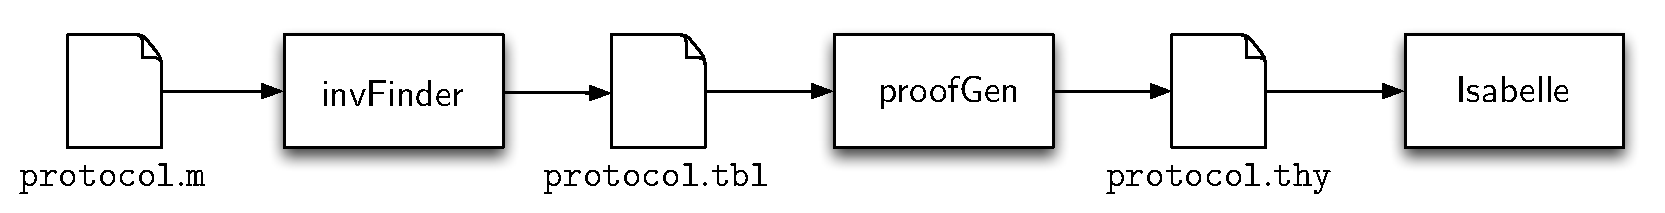
\includegraphics[width=1\textwidth]{paraVerifier.pdf}
\vspace{-20pt}
\caption{The workflow of {\sf paraVerifier} \label{fig:archParaVerifier}
}
\end{figure}
\vspace{-20pt}
\paragraph{invFinder}%In order to verify  that an
%invariant $inv$ holds for any parameterizd instance of a protocol.
Given a protocol $\mathcal{P}$ and a property $inv$,  written in
a Murphi  file {\tt prot.m}, is compiled into an internal form {\sf prot.ml}, then fed into the
\texttt{invFinder}. {\tt invFinder} automatically transforms the Murphi file into the internal formal model in Ocaml, then tries to find useful auxiliary invariants and causal relations which are capable of proving $inv$. To construct auxiliary invariants and causal relations, we employ heuristics inspired by consistency relation. Also, when several candidate invariants are obtained using the heuristics, we use oracles such as NuSMV and Murphi model checker and an SMT-solver to check each of them under a small reference model of $\mathcal{P}$, and chooses the one that has been verified in the oracles. A table {\tt prot.tbl} is worked out  to store the set of ground invariants and
 causal relations.


\paragraph{proofGen} For the auxiliary invariants and causal relations stored in table {\tt prot.tbl}, {\tt proofGen} generalizes them  into  parameterized forms, which are then used to construct a completely parameterized formal proof in a theorem prover (e.g., Isabelle) to model $\mathcal{P}$ and to prove the property $inv$. After the base theory is imported, the generated proof is checked automatically.  Usually, a proof is done interactively. Special efforts in the design of the proof generation are made in order to make the proof checking automatically.




%\vspace{-0.2cm}
\section{Informal Account of FLASH Protocol\label{sec:informalOfFLASH}}
%\vspace{-0.2cm}
%\subsection{A textual description}
\paragraph*{A textual description}Firstly we give a classical textual description, which is directly cited from the material in \cite{Park2000} to informally introduce FLASH protocol.
FLASH protocols is a directory-based one which supports a large number of distributed processing nodes. Each cache line-sized block in memory is associated with directory header which keeps information about the \bedt{cache} line. Each memory address has a home node. Each cache line-sized block in memory is associated
with a directory header which keeps information about the \bedt{cache} line. For a memory \bedt{address}, the
node on which that piece of memory is physically located is called the home; the other
nodes are called remote. The home maintains all the information about memory in
its main memory in the corresponding directory headers.
The system consists of a set of nodes, each of which contains a processor, caches, and
a portion of the global memory. The distributed nodes communicate using asynchronous
messages through a point-to-point network. The state of a cached copy is in either invalid,
shared (readable), or exclusive (readable and writable). There are typical kinds of transactions as follows:\\%\begin{description}%\item[READ-Transaction]
\noindent{\bf READ-Transaction} If a read miss occurs in a processor where the state of its cache is invalid, the corresponding node sends out a GET request to the
home (this step is not necessary if the requesting processor is in the home). Receiving the
GET request, the home consults the directory corresponding to the memory line to decide
what action the home should take. If the line is pending, meaning that another request
is already being processed, the home sends an NAK (negative acknowledgment) to the
requesting node. If the directory indicates there is a dirty copy in a remote node, then the
home forwards the GET to that node. Otherwise, the home grants the request by sending
a PUT to the requesting node and updates the directory properly. When the requesting
node receives a PUT reply, which returns the requested memory \bedt{address}, the processor sets
its cache state to shared and proceeds to read.\\%\item[WRITE-Transaction]
\noindent{\bf WRITE-Transaction} For a write miss, the corresponding node sends out a GETX request to the home.
Receiving the GETX request, the home consults the directory. If the \bedt{cache} line is pending,
the home sends an NAK to the requesting node. If the directory indicates there is a dirty
copy in a third node, then the home forwards the GETX to that node. If the directory
indicates there are shared copies of the memory \bedt{address} in other nodes, the home sends
INVs (invalidations) to those nodes. At this point, the protocol depends on which of two
modes the multiprocessor is running in EAGER or DELAYED. In EAGER mode, the home
grants the request by sending a PUTX to the requesting node; in DELAYED mode, this
grant is deferred until all the invalidation acknowledgments are received by the home. If
there are no shared copies, the home sends a PUTX to the requesting node and updates
the directory properly. When the requesting node receives a PUTX reply which returns
an exclusive copy of the requested memory \bedt{address}, the processor sets its cache state to
exclusive and proceeds to write.

%\vspace{-10pt}

Usually, only an \bedt{(in)formal}  account of FLASH protocol, as shown above, is provided in most previous work.   It is still not very clear to most readers. %, especially in the novel who are not very familiar with FLASH protocol.
Its is very desirable for people to have some flow-charts each of  which is a series of rules executed to complete a READ/WRITE transaction. Such a flow shows: Who do execute transition rules? How  are rules executed in some special causal order to finish a transaction? How are transactions of different nodes  synchronized with some mechanism to guarantee  important properties? %Here we adopt a novel data flow chart to illustrate a case of READ (or WRITE) transaction.%, as shown below:  and exchange messages to implement the designed protocol goals.



%\subsection{A Flow Chart}
\paragraph*{A Flow Chart} Formally, a transaction flow is a structure, which can be formalized by a pair $<R \times N, \rightarrow \cup \Rightarrow>$, where $(r,i) \in R \times N$ is a  node, indicating that a client $i$ performs an action of executing a rule $r$. Relations  $\rightarrow$  and $\Rightarrow$ are two   orders over $R \times N$. $(r_1,i_1) \rightarrow (r_2,i_2) \equiv \exists v~e. (v:=e) \in \mathsf{act}(r_1) \land (v=e) \in decompose(guard(r_2))$. Here $v:=e$ is an assignment; $\mathsf{act}$ is the set of assignments of an action of a rule; A formula $f$ in conjunction form can be composed of a set of sub-formulas $f_i$, denoted as $decompose(f)$, such that each $f_i$  is not of a conjunction form and $f$ is semantically equivalent to $f_1 \land f_2 \land ... \land f_N$. Intuitively $(r_1,i_1) \rightarrow (r_2,i_2)$ means that the triggering of agent $i_2$ executing $r_2$ needs the completion of agent $i_1$ executing $r_1$; $(r_1,i_1) \Rightarrow (r_2,i_1)$ means that agent $i_1$'s action of executing $r_2$ follows the completion of  executing $r_1$. A classical three-hop flow case of an READ-transaction including a sharing-write back is shown as follows:

\vspace{-20pt}
\begin{figure}[htbp]
\centering
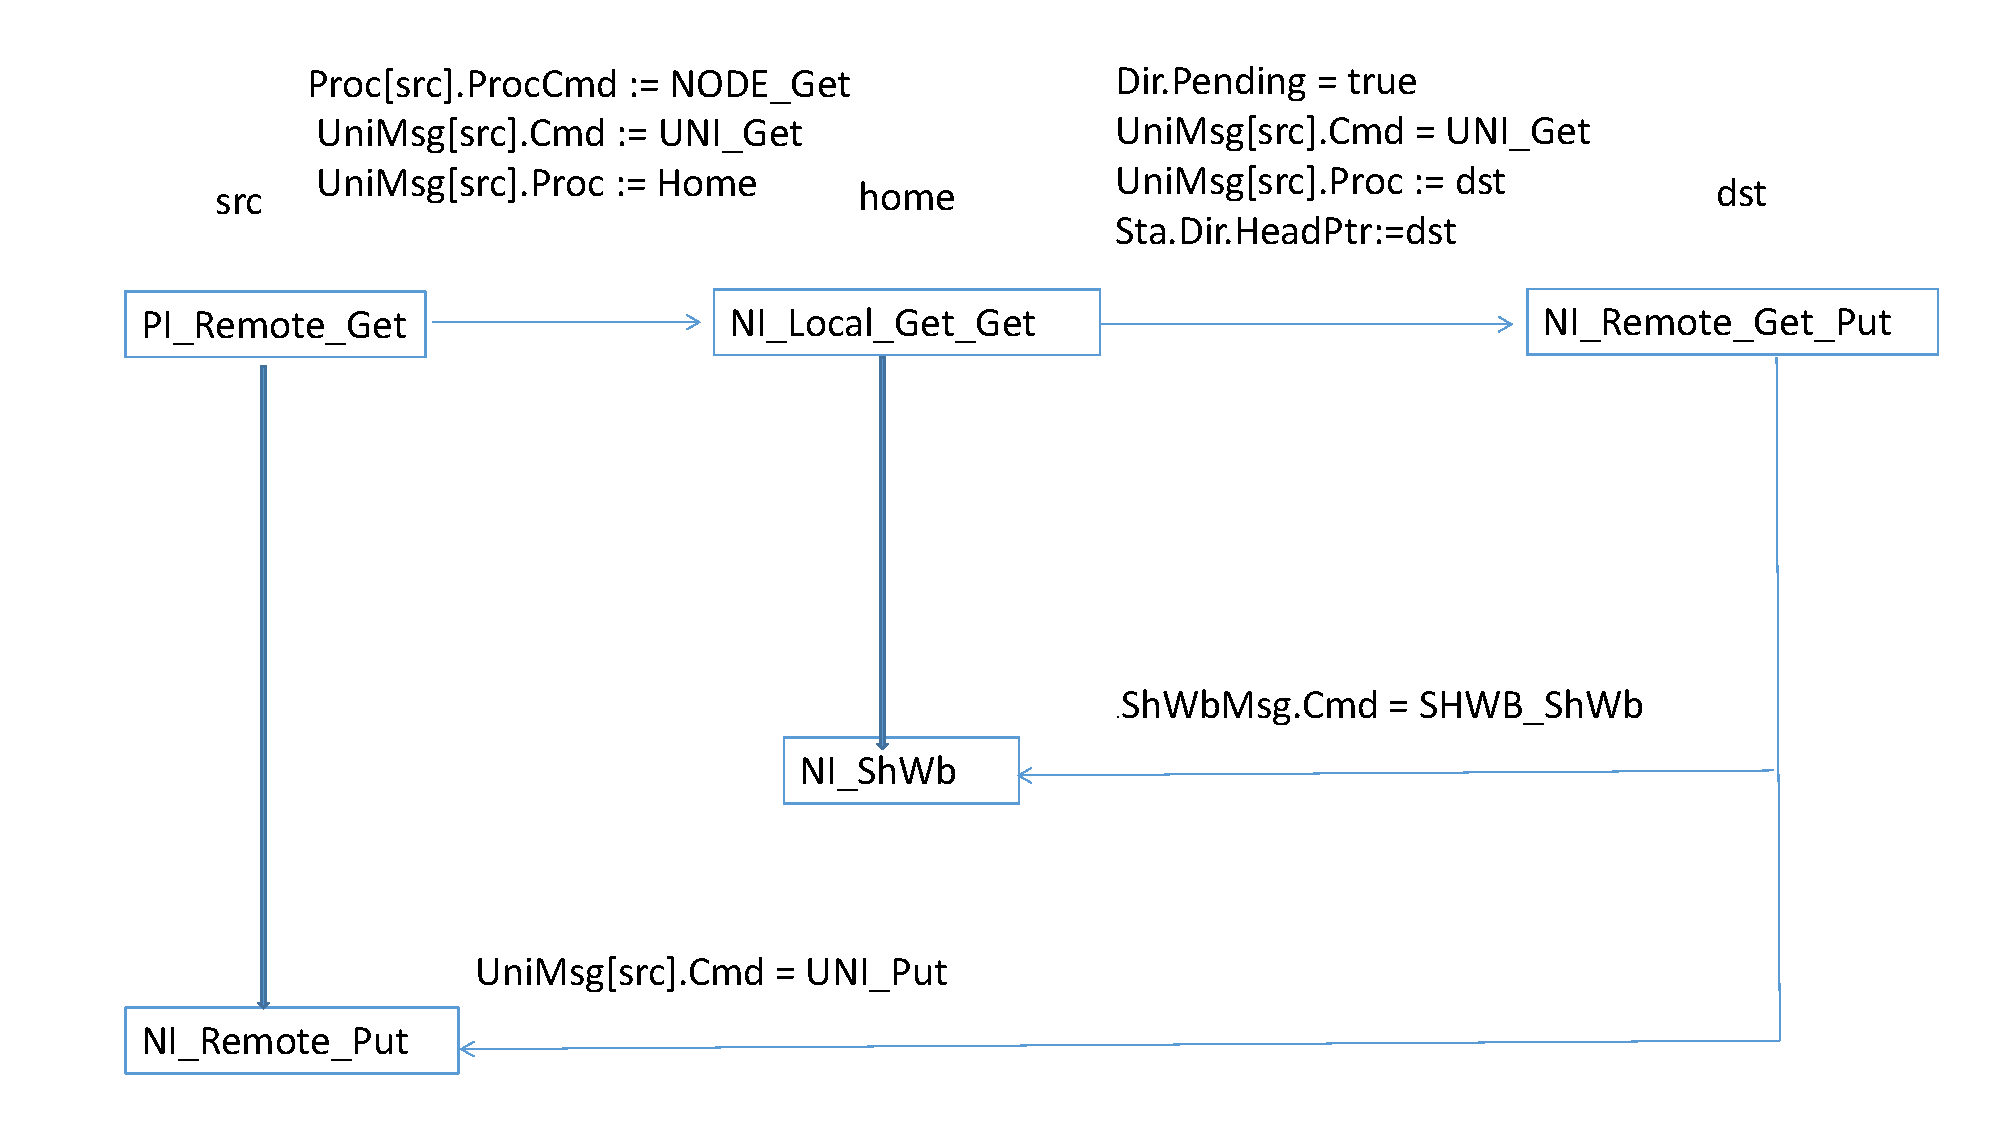
\includegraphics[width=0.8\textwidth]{flow2.pdf}
\vspace{-20pt}
\caption{The flow of READ-transaction including a sharing-write back\label{fig:arch}}
\end{figure}
\vspace{-15pt}

This flow is finished by the following steps:
\begin{enumerate}[noitemsep,nolistsep]
\item An idle remote  client $src$ needs a shared copy of a memory line, executes   rule PI\_Remote\_Get, and  sends the GET request to home.

\item  When the GET request from $src$ arrives at the
home, the home consults the directory to find that the line is dirty in $dst$,  executes rule NI\_Lcal\_Get\_Get: forwards the GET to $dst$ by telling that $src$ needs the data, and sets Dir.Pending TRUE to make no any other node's request to be processed during the sharing write-back procedure.

\item  When $dst$ receives the forwarded GET, the
processor $dst$ executes rule \\
NI\_Remote\_Get\_Put, sets its copy to shared state and issues a PUT to $src$ conveying the dirty data,  and  issues a   shwb\_shwb
 (sharing write-back) conveying the dirty data at the same time.

\item   When $home$ receives this SHWB message, it executes the rule NI\_ShWb, and
 writes the
data back  to main memory and puts $src$ on the sharers' list.

\item When $dst$ receives this PUT message, it executes the rule NI\_Remote\_Put. If there is not another INV message, then it   uses the received data to update its cache line and sets its cache to shared state.


\end{enumerate}

Compared with a textual description, a flow description has the advantage that (1) causal order relations between agents' executing rules are illustrated clearly; (2) communications between agents are also illustrated. In section \ref{sec:experiments} and \ref{sec:relatingWithFlow} we combine steps in a flow with auxiliary inductive invariants, by which we can make it clear that how  FLASH protocol guarantee the synchronization between different clients. Formally, auxiliary inductive invariants will show    the synchronization mechanism in logical formulas. It is also noteworthy that the purpose about the flow in our paper is completely different with \cite{Talupur2008a}. In \cite{Talupur2008a}, the flow message is recognized by people manually and is used as flow invariants to assist the verification. As comparison, we extract the flow knowledge  to help user better understanding the system with the generated invariants.

%Usually, the above informal paper account of
%\begin{description}
%\item[(1)]  In most previous papers on FLASH protocol, only informal accounts as shown above are discussed. It is still not very clear to most readers, especially to the novel who are not very familiar with FALSH. Its is very desirable for people to have some flow-charts each of  which is a series of rules executed to complete a READ/WRITE transaction. From such a flow, how rules are executed in some special causal order to finish a transaction? How do transactions of different nodes are synchronized with some mechanism to guarantee  the consistency property?

%\item[(2)] It is preferable to combine steps in a flow with auxiliary inductive invariants. From this we can make it clear that how key state variables in the directory of FLASH protocol guarantee the synchronization between different nodes. Formally, auxiliary inductive invariants will show    the synchronization mechanism in logical formulas.
% \end{description}




%=========================================
\section{Formal Description of FLASH protocol in Murphi\label{sec:formalDescription}}
%=========================================
A formal protocol model includes a set of parameterized transition rules and properties.  Here we adopt a version of FLASH protocol similar to that in \cite{cubeicBeyond}, which is different from the version in \cite{Chou2004}. The difference between them lies in the modeling of behaviors of a Home node. Behaviours of the Home node is not identical to those of the other nodes while behaviors of
 a non-Home node are identical to those of the other non-Home node. In the model of work in \cite{Chou2004}, state variables of the Home node and non-Home nodes are both array-variables. This modeling has a shortage of destroying the symmetry between indices which represents identifiers for agents.

In our modeling, the symmetry between indices should be preserved and will be used in {\sf paraVerifier}. Namely,  %a  state variable $a$ on non-Home nodes are stored in array-variables.
some parameterized variable $a[i]$ records some state  $a$ of node $i$. Home is not an explicit index to reference a node in our model. State variable
  $a$ of the Home node  is recorded as a global  (or non-parameterized) variable $Homea$. %Index variable $v$ to represent some index of a node is only for non-Home nodes. We explicitly introduce an extra variable $Homev$ to identify the case when the node index should be $Home$.
 Being consistent with the above philosophy, our FLASH protocol in Murphi is changed accordingly. For instance, we compare the original version in \cite{Chou2004}, which is shown in (a), with our version, which is shown in (b):

%\forget{
%\vspace{-5pt}
\begin{specification}
\begin{minipage}[t]{0.5\linewidth}
 UNI\_MSG : record\\
\twoSpaces    Cmd : UNI\_CMD;\     Proc : NODE;\\
\twoSpaces     Data : DATA;\\
  end;\\

 DIR\_STATE : record\\
\twoSpaces     Pending : boolean;\     Local : boolean;\\
\twoSpaces     Dirty : boolean;\      HeadVld : boolean;\\
\twoSpaces     HeadPtr : NODE;\\
\twoSpaces     ShrVld : boolean;\\
\twoSpaces     ShrSet : array [NODE] of boolean;\\
\twoSpaces     InvSet : array [NODE] of boolean;\\
  end;  \\

  ruleset src : NODE do\\
rule "PI\_Remote\_Get"\\
  src != Home \&\\
  Sta.Proc[src].ProcCmd = NODE\_None \&\\
  Sta.Proc[src].CacheState = CACHE\_I\\
==>\\

begin\\
\twoSpaces    Sta.Proc[src].ProcCmd := NODE\_Get;\\
\twoSpaces    Sta.UniMsg[src].Cmd := UNI\_Get;\\
\twoSpaces    Sta.UniMsg[src].Proc := Home;\\
endrule;\\
endruleset;
\center (a)\\
\twoSpaces \\
\end{minipage}

%\begin{specification}{0.5\linewidth}
\begin{minipage}[t]{0.4\linewidth}

UNI\_MSG : record\\
\twoSpaces     Cmd : UNI\_CMD;\     Proc : NODE;\\
\twoSpaces     HomeProc : boolean;\       Data : DATA;\\
  end;\\


  DIR\_STATE : record\\
\twoSpaces     Pending : boolean;\     Local : boolean;\\
\twoSpaces     Dirty : boolean;\      HeadVld : boolean;\\
\twoSpaces     HeadPtr : NODE;\      HomeHeadPtr : boolean;\\
\twoSpaces     ShrVld : boolean;\\
\twoSpaces     ShrSet : array [NODE] of boolean;\\
\twoSpaces     HomeShrSet : boolean;\\
\twoSpaces     InvSet : array [NODE] of boolean;\\
\twoSpaces     HomeInvSet : boolean;\\
  end;\\

  ruleset src : NODE do\\
rule "PI\_Remote\_Get"\\
\twoSpaces   Sta.Proc[src].ProcCmd = NODE\_None \&\\
\twoSpaces   Sta.Proc[src].CacheState = CACHE\_I\\
==>\\
begin
\twoSpaces   Sta.Proc[src].ProcCmd := NODE\_Get;\\
\twoSpaces   Sta.UniMsg[src].Cmd := UNI\_Get;\\
\twoSpaces   Sta.UniMsg[src].HomeProc := true;\\
endrule; endruleset;
\center (b)\\
\twoSpaces \\
\end{minipage}
\end{specification}
%}







\forget{
\begin{multicols}{2}
\begin{specification}\\
 UNI\_MSG : record\\
\twoSpaces    Cmd : UNI\_CMD;\     Proc : NODE;\\
\twoSpaces     Data : DATA;\\
  end;\\

 DIR\_STATE : record\\
\twoSpaces     Pending : boolean;\     Local : boolean;\\
\twoSpaces     Dirty : boolean;\      HeadVld : boolean;\\
\twoSpaces     HeadPtr : NODE;\\
\twoSpaces     ShrVld : boolean;\\
\twoSpaces     ShrSet : array [NODE] of boolean;\\
\twoSpaces     InvSet : array [NODE] of boolean;\\
  end;  \\

  ruleset src : NODE do\\
rule "PI\_Remote\_Get"\\
  src != Home \&\\
  Sta.Proc[src].ProcCmd = NODE\_None \&\\
  Sta.Proc[src].CacheState = CACHE\_I\\
==>\\

begin\\
\twoSpaces    Sta.Proc[src].ProcCmd := NODE\_Get;\\
\twoSpaces    Sta.UniMsg[src].Cmd := UNI\_Get;\\
\twoSpaces    Sta.UniMsg[src].Proc := Home;\\
endrule;
endruleset;\\
\end{specification}\\
\twoSpaces \twoSpaces \twoSpaces \center(a)
\columnbreak

\begin{specification}\\
UNI\_MSG : record\\
\twoSpaces     Cmd : UNI\_CMD;\     Proc : NODE;\\
\twoSpaces     HomeProc : boolean;\       Data : DATA;\\
  end;\\


  DIR\_STATE : record\\
\twoSpaces     Pending : boolean;\     Local : boolean;\\
\twoSpaces     Dirty : boolean;\      HeadVld : boolean;\\
\twoSpaces     HeadPtr : NODE;\      HomeHeadPtr : boolean;\\
\twoSpaces     ShrVld : boolean;\\
\twoSpaces     ShrSet : array [NODE] of boolean;\\
\twoSpaces     HomeShrSet : boolean;\\
\twoSpaces     InvSet : array [NODE] of boolean;\\
\twoSpaces     HomeInvSet : boolean;\\
  end;\\

  ruleset src : NODE do\\
rule "PI\_Remote\_Get"\\
\twoSpaces   Sta.Proc[src].ProcCmd = NODE\_None \&\\
\twoSpaces   Sta.Proc[src].CacheState = CACHE\_I\\
==>\\
begin
\twoSpaces   Sta.Proc[src].ProcCmd := NODE\_Get;\\
\twoSpaces   Sta.UniMsg[src].Cmd := UNI\_Get;\\
\twoSpaces   Sta.UniMsg[src].HomeProc := true;\\
endrule; endruleset;
\end{specification}\\
\twoSpaces \twoSpaces \twoSpaces \center(b)
\end{multicols}
}

%The above is the version in \cite{}, while our version is as follows:

%\vspace{-0.8cm}

In our version, we add a field $HomeProc$. If $HomeProc$ is true, then this is according to the case $Proc=Home$ in the original version, else     the case where $Proc$ is a non-Home one. $HomeHeadPtr$ is added similarly in our model.  $HomeShrSet$  and     $HomeInvSet$ are added in order to model $ShrSet[Home]$ and $InvSet[Home]$ to be true in the original version. We use the assignment $Sta.UniMsg[src].HomeProc := true$ to  model   that $Sta.UniMsg[src].Proc$ is the $Home$ node. There are three properties under verification. Our experiment data includes the
${\sf paraVerifier}$ instance, invariant sets, Isabelle proof
scripts \cite{LiCache16a}.

\begin{specification}\\
invariant "CacheStateProp"\\
  forall p : NODE do forall q : NODE do     p != q ->\\
    !(Sta.Proc[p].CacheState = CACHE\_E \& Sta.Proc[q].CacheState = CACHE\_E)\\
  end end;\\

invariant "CacheStatePropHome"\\
  forall p : NODE do\\
    !(Sta.Proc[p].CacheState = CACHE\_E \& Sta.HomeProc.CacheState = CACHE\_E)\\
  end;\\

invariant "MemDataProp"\\
  !((Sta.Dir.Dirty = FALSE) \& (!(Sta.MemData = Sta.CurrData)));\\
\end{specification}\\

The former two properties are the mutual-exclusion properties between  cache state status of two nodes. The last is the  data property.

%=========================================
\section{Verifying FLASH protocol by {\sf paraVerifer} \label{sec:experiments}}
\paragraph{An obstacle of generating an SMV-oracle and its solution}
For cache coherence protocols like MESI or German protocols with small scales,   {\sf paraVerifier}  is easy to use to verify automatically them. \bedt{A model written in Murphi language} is provided as a formal model, which contains both the protocol and properties under verification. The Murphi model will be automatically transformed into not only an internal model but also an SMV-model. NuSMV will \bedt{be used as the model checking engine} and be called to compute the reachable set of the SMV-model. The internal model will be used by the {\sf invFinder} to generate auxiliary invariants. During this generation procedure, a set of candidate invariant formulas are generated in one step, and only one is chosen  if it is an invariant by checking the reachable set of   SMV-model. The oracle of the SMV-model is automatically generated inside the {\sf inVfinder} without human intervention.

However, FLASH protocol with data path is a real world protocol with industry scale. For a FLASH protocol   instance configuration size NODENUM=3 and DATANUM=2, the protocol is so complex that NuSMV can't compute the reachable state set of the SMV-model which is generated by {\sf invFinder} in a computing server  with 32 Inter Xeon processors, 384 GB memory. In fact, this problem of  state explosion is the main obstacle to the applying previous automatic solutions such as \cite{Arons2001,Lv2007} to the parameterized verification of FLASH protocol. For instance, a reachable state set of a protocol instance of FLASH protocol is needed in both the work in \cite{Arons2001,Lv2007}. The former needs the reachable state set to compute the so-called ``invisible inductive invariants" for deductive theorem proving. The latter needs it to strengthen
 the guards of rule for a counter-example guided refinement of an abstract protocol. Due to the non-availability of the necessary the reachable state set of a proper instance of FLASH protocol, the above two approaches both fail.

 In order to overrun the obstacle of oracles, {\sf invFinder} provides techniques of simplifying protocols and hybrid oracles. For a complex protocol, a smv-model of a  simplified version of this protocol can be used as an external oracle to verify the guessed candidate formulas. For FLASH protocol with data paths,  we construct a SMV -model of a simplified version of the FLASH protocol without data paths, and use NuSMV to enumerate its reachable state set to judge a candidate invariant formula. Here we  emphasize that the reachable state set of the simplified FLASH protocol  instance  with configuration size NODENUM=3 can be enumerated by the NuSMV in the aforementioned computing server. This oracle is enough for the {\sf invFinder} to find all the invariant formulas on control variables (or without data properties).

 However, if a candidate invariant formula in which data variables occurring, how does {\sf invFinder} deal with it?  For instance, ((Sta.Dir.Dirty = FALSE) \& (!(Sta.MemData = Sta.CurrData))) can't be judged via the SMV -model of a simplified version of the FLASH protocol without data paths. At this time, a hybrid oracle will be used.  A full protocol instance in Murphi  with configuration size NODENUM=3 ana DATANUM=2 \bedt{is built}, and  Murphi \bedt{tool} is run to judge the formula containing data variables. Here we adopt an \bedt{heuristic} strategy: \bedt{if Murphi tool has been running to check the property up to a time-out,} and no counter-example is found, then the checked formula will be regarded for an invariant.

 The \bedt{heuristic} may introduce a false invariant, which leads to a doubt of the soundness of our method.  Intuitively, a  false invariant holds at any   state which either occurs in the reachable state set of the SMV-model or in a state traversed by Murphi. But it may not hold at a state of a protocol instance which is not in the aforementioned reachable state sets. Here we emphasize that the ultimate correctness is guaranteed by the theorem proving process of the generated proof script in Isabelle. If such a false invariant is generalized and occurs in the parameterized invariant set, the generated proof script can't be passed in Isabelle.

\vspace{-10pt}
\paragraph{Verifying \bedt{procedure}}  In order to verify FLASH protocol by {\sf paraVerifier} under Linux system, some simple steps are needed.

\begin{enumerate}[noitemsep,nolistsep]
\item The Murphi model of FLASH protocol is converted to its corresponding internal model by compiler {\sf murphi2ocaml}.
\item The specific verifier for FLASH protocol with OCaml is built. Furthermore, the generated executable file is  executed on a server while a model checking engine for NuSMV oracle and a model checking engine for Murphi oracle are executed on other servers respectively. Afterwards, a directory containing proof scripts will be generated.
\item The proof scripts in Isabelle is then executed.
\end{enumerate}

\forget{
Firstly, we convert Murphi model of FLASH protocol to its corresponding internal model by compiler {\sf murphi2ocaml} supposing that the compiler was put in path {\sf\$\{moc\}}.

\begin{specification}
  \$ python \$\{moc\}/gen.py -m flash.m > flash.ml
\end{specification}

Secondly, we build the specific verifier for FLASH protocol with OCaml and run the generated executable file supposing that address of the NuSMV oracle was {\sf vserv} and address of the Murphi oracle was {\sf mserv}. Afterwards, a directory named {\sf n\_flash} where proof scripts were put will be generated.

\begin{specification}
  corebuild flash.byte -pkg re2 -I src\\
  ./flash.byte -vh vserv -mh mserv
\end{specification}

Finally, we run the proof scripts in Isabelle.

\begin{specification}
  cd n\_flash\\
  ./run.sh
\end{specification}
}




We run {\sf paraVerifier} on a client with 4 Intel Xeon processors, 8 GB memory and 64 bit Linux 3.15.10. The NuSMV oracle and Murphi oracle were set on a server with 32 Inter Xeon processors, 384 GB memory and 64 bit Linux 2.6.32. Result of our experiments is as Table \ref{tab:flashRes}.


%\vspace{-10pt}
\begin{table}[!htbp]
  \centering
  \footnotesize
   \caption{Verification Result on FLASH protocol}
  \label{tab:flashRes}
  \vspace{-5pt}
  \begin{tabular}{|c|c|}
    \hline
    \#rules & 62\\
    \hline
    \#invariants & 162\\
    \hline
    Time of {\sf paraVerifier} (minutes) & 9.82\\
    \hline
    Memory of {\sf paraVerifier} (MB) & 178\\
    \hline
    Time of proof (hours) & 10.76\\
    \hline
  \end{tabular}

\end{table}
%\vspace{-10pt}





%=========================================
%\subsection{Auxiliary Invariants and Causal Relations}\label{sec:causal lines}
%=========================================
%Initially, {\sf paraVerifier} sets the auxilary invariant set to be {\tt \{!(Sta.Proc[1].CacheState = CACHE\_E \& Sta.Proc[2].CacheState = CACHE\_E),
%!(Sta.Proc[1].CacheState = CACHE\_E \& Sta.HomeProc.CacheState = CACHE\_E), !((Sta.Dir.Dirty = FALSE) \& (!(Sta.MemData = Sta.CurrData)))\}}.

%We also need tell  the tool two protocol instances. One is with size 2 but without data paths (i.e., the variables such as Sta.MemData and Sta.CurrData can be omitted), and the second is with size 2 but with data paths.
%The reachable state set of the former can be enumerated by SMV, but that of the latter cann't be. {\sf paraVerifier} need the two instances to verify a candidate formula which is guessed by heuristics. If all the variables occurring in the candidate formula is  in the former instance, then {\sf paraVerifier} will query the   reachable state set to verify the formula; otherwise {\sf paraVerifier} will call MURPHI to verify the formula. In the second kind of checking, a time limit will beset, if MURPHI can check the falsity of the formula within the limit, then the candidate will be dropped; otherwise the candidate will be put it into the auxiliary invariant set.

\vspace{-10pt}

\paragraph{Auxiliary Invariants }
The set of auxiliary invariants, which is found by {\sf paraVerifier}, contains 162 formulas. This work is  fully AUTOMATICALLY  done by {\sf paraVerifier}.  Here we select and analyze all the invariants on Sta.Dir.Pending, which help us to understand the function of the control variable.

\begin{specification}
inv\_\_44!((Sta.HomeUniMsg.Cmd = uni\_get) \& (Sta.Dir.Pending = FALSE))\\
inv\_\_52!((Sta.HomeUniMsg.Cmd = uni\_getx) \& (!(Sta.Dir.Pending = TRUE)))\\
inv\_\_53!((Sta.HomeUniMsg.Cmd = uni\_put) \& (!(Sta.Dir.Pending = TRUE)))\\
inv\_\_57!((Sta.HomeUniMsg.Cmd = uni\_putx) \& (!(Sta.Dir.Pending = TRUE)))\\
inv\_\_59!((Sta.UniMsg[1].Cmd = uni\_get) \& (Sta.UniMsg[1].HomeProc = FALSE) \& (Sta.Dir.Pending = FALSE))\\
inv\_\_74!((Sta.UniMsg[1].Cmd = uni\_getx) \& (Sta.UniMsg[1].HomeProc = FALSE) \&(!(Sta.Dir.Pending = TRUE)))\\
inv\_\_88!((Sta.Dir.InvSet[1] = TRUE)  \& (Sta.UniMsg[2].Cmd = uni\_putx)\& (Sta.Dir.Pending = FALSE))\\
inv\_\_91!((Sta.ShWbMsg.Cmd = shwb\_shwb) \& (!(Sta.Dir.Pending = TRUE)))\\
inv\_\_92!!((Sta.ShWbMsg.Cmd = shwb\_fack) \& (Sta.Dir.Pending = FALSE))\\
inv\_\_111!((Sta.NakcMsg.Cmd = nakc\_nakc) \& (Sta.Dir.Pending = FALSE))\\
inv\_\_114!((Sta.Dir.InvSet[1] = TRUE) \& (Sta.Dir.Dirty = TRUE) \& (Sta.Dir.Pending = FALSE))\\
inv\_\_117!((Sta.Dir.InvSet[1] = TRUE)  \& (Sta.Dir.HeadVld = FALSE)\& (Sta.Dir.Pending = FALSE))\\
inv\_\_134!((Sta.Dir.InvSet[1] = TRUE)  \& (Sta.Proc[2].CacheState = cache\_e)\& (Sta.Dir.Pending = FALSE))\\
inv\_\_153!((Sta.Dir.InvSet[1] = TRUE) \& (Sta.WbMsg.Cmd = wb\_wb) \& (Sta.Dir.Pending = FALSE))\\
inv\_\_161!((Sta.HomeProc.CacheState = cache\_s) \& (Sta.Dir.Pending = TRUE))\\
\end{specification}

From these invariants, we can know when the control state variable Sta.Dir.Pending is set or not. In the following analysis, an index 1 can be generalized into any index in one invariant,  two indices 1 and 2 can be generalized into any two indices $i_1$ and $i_2$ s.t. $i_1 \neq i_2$.
\vspace{-0.2cm}
\begin{itemize}
 \item Invariant 44 means that the Home node is fetching a data from some node to read, thus {\tt (Sta.HomeUniMsg.Cmd = uni\_get)}, so the pending flag is  TRUE to block another new READ-WRITE request.
 \item Invariants 52, 53, and 57 can be analyzed similarly.
 \item In invariant 59, {\tt (Sta.UniMsg[1].Cmd = uni\_get) \& (Sta.UniMsg[1].Home} {\tt Proc = FALSE)} means that node 1 has request a shared copy and been granted to fetch the copy from some node, thus Sta.UniMsg[1].HomeProc = FALSE, the pending flag is set TRUE to block another new READ-WRITE requests.
  \item    Invariant 74 has a similar meaning while the request is for WRITE operation.

  \item    Invariant 88 specifies that node 2 performs a write-request, thus {\tt Sta.UniMsg} {\tt[2].Cmd = uni\_putx}, and the data is shared by node 1, then the shared copy in node 1 is invalidated, thus (Sta.Dir.InvSet[1] = TRUE), at this time,  the pending flag is set TRUE to block another new READ-WRITE request.

  \item   Invariants 91 and 92 says that this flag is set during sharing write-back procedure. Invariants 111  that this flag is set during the nakc procedure when  Sta.NakcMsg.Cmd = NAKC\_Nakc.

   \item     Invariants 114 that the flag is set during the invalidating procedure to an old shared-copy store in node 1. The invalidating procedure is a sub-procedure  of a WRITE request from any other node. In 134, {\tt Sta.Proc[2].CacheState = cache\_e} shows that the WRITE request is from node 2, and CacheState of node 2 changes to exclusive even before node 1 has not been invalidated. From this, we can see that the version we verify is an eager-mode.

   \item       Invariant 153 that Sta.Dir.Pending is set during a write-back procedure.

  \item  The last one says that if there is a  local shared copy in the Home node, Sta.Dir.Pending is FALSE because the   requests can be processed at once, thus, the system need not be pend.
\end{itemize}
Not only auxiliary invariants are searched, but also causal relations between   invariants and  rules are searched. A fragment on the rule {\tt NI\_Remote\_PutX} and invariant {\tt inv1= !((Sta.Proc[2].CacheState = cache\_e) \& (Sta.Proc[1].\ \\CacheState = cache\_e))} is shown as below:\\
%table.%=========================================%\subsection{ Parameterized Proof Script}%=========================================
\vspace{-0.3cm}

%\begin{minipage}[t]{0.4\textwidth}
\begin{specification}
ruleset dst : NODE do rule "NI\_Remote\_PutX"\\
  Sta.UniMsg[dst].Cmd = UNI\_PutX \&  Sta.Proc[dst].ProcCmd = NODE\_GetX ==>\\
%==>\\
begin   Sta.UniMsg[dst].Cmd := UNI\_None;  Sta.Proc[dst].ProcCmd := NODE\_None;\\
  Sta.Proc[dst].InvMarked := false;   Sta.Proc[dst].CacheState := CACHE\_E;\\
  Sta.Proc[dst].CacheData := Sta.UniMsg[dst].Data;\\
endrule; endruleset;\\\\
1 rule: NI\_Remote\_PutX[1]; inv: !((Sta.Proc[2].CacheState = cache\_e) \& (Sta.Proc[1].CacheState\\ = cache\_e)); g: TRUE;
rel: invHoldForRule3-inv4:!((Sta.Proc[2].CacheState = cache\_e) \& \\(Sta.UniMsg[1].Cmd = uni\_putx))\\
2 rule: NI\_Remote\_PutX[2]; inv: !((Sta.Proc[2].CacheState = cache\_e) \& (Sta.Proc[1].CacheState\\ = cache\_e)); g: TRUE;
rel: 3invHoldForRule3-inv4:!((Sta.Proc[1].CacheState = cache\_e) \& \\(Sta.UniMsg[2].Cmd = uni\_putx))\\
3 rule: NI\_Remote\_PutX[3]; inv: !((Sta.Proc[2].CacheState = cache\_e) \& (Sta.Proc[1].CacheState\\ = cache\_e)); g: TRUE;
 rel: invHoldForRule2
\end{specification}

\begin{itemize}[noitemsep,nolistsep]
\item Line 1 specifies that if a state $s$ satisfies the guard of the rule, and %{\tt inv4}
  {\tt inv4= !((Sta.Proc[2].CacheState=cache\_e)\&(Sta.UniMsg[1].Cmd=uni\_putx))}, and $s'$ is the post state after the execution of the rule, then the invariant {\tt inv1} holds at state $s'$. Reader can verify this easily. This expresses the intuition behind the  relation $invHoldForRule_3$. Line 2 can be analyzed similarly.
 \item Line 3 that {\tt NI\_Remote\_PutX[3]} has nothing to do with all the variables in {\tt inv1}, thus $s$ satisfies the formula if and only the post state   $s'$ satisfies the formula. This expresses the intuition behind the   relation $invHoldForRule_2$.
\end{itemize}%There are ? lines in the causal relation
%\end{minipage}

\vspace{-10pt}
\paragraph{Parameterized Proof Script} There are concrete invariants and causal relations, where each  index is a concrete one such as 1 and 2, etc. {\tt proofGen} generalizes these into an N-parameterized form, where each index is symbolic such as $i1$ and $i2$ and $N$ is also symbolic. An Isabelle proof script is  generated by {\tt proofGen}, where an N-parameterized instance of FLASH protocol is modeled   and the properties are formally proved. The Hierarchy of the lemmas is illustrated in Fig. \ref{fig:lemmaHierachy}. %$A \rightarrow B$ means that the proof of lemma $A$ needs applying lemma $B$.


%\vspace{-20pt}

\begin{figure}[htbp]
\centering %


\includegraphics[width=0.8\textwidth]{thy.pdf}
\vspace{-20pt}
\caption{The Hierachy of the lemmas\label{fig:lemmaHierachy}
}
\end{figure}

%\vspace{-3pt}
\begin{specification}\\
definition inv1::"nat $\Rightarrow$ nat $\Rightarrow$ formula" where [simp]:\\
"inv1 \pInv0 \pInv1 $\equiv$
(neg (andForm (eqn (IVar (Field (Para (Field (Ident ''Sta'') ''Proc'') \pInv1)\\ ''CacheState''))\\
 (Const CACHE\_E)) (eqn (IVar (Field (Para (Field (Ident ''Sta'') ''Proc'') \pInv0)\\ ''CacheState'')) (Const CACHE\_E))))"\\
definition invariants::"nat $\Rightarrow$ formula set" where [simp]:\\
"invariants N $\equiv$ \{f.
($\exists$ pInv0 pInv1. pInv0$\le$N$\wedge$pInv1$\le$N$\wedge$pInv0~=pInv1$\wedge$f=inv1  pInv0 pInv1) $\vee$\\
($\exists$ pInv0. pInv0 $\le$N$\wedge$f=inv2  pInv0) $\vee$
(f=inv3  ) $\vee$ ......\\
($\exists$ pInv0. pInv0$\le$N$\wedge$f=inv162  pInv0) \}"\\
\end{specification}\\
%\vspace{-10pt}

%In detail, the proof script is divided into   parts as follows:
%\begin{enumerate}[noitemsep,nolistsep]
%\item[1] Definitions of formally parameterized invariant formulas, which are generalized from concrete invariants. There are 162 such invariants. An actual N-parameterized invariant can be obtained by instantiating a formal invariant formula with symbolic indexes. All   actual invariant formulas in the N-parameterized are defined by a set invariants N;

%\item[2] Definitions of formally parameterized rules,  which can be directly transformed from the  Murphi rules of FLASH protocol. There are 62 rules.  Actual parameterized rules can be defined similarly. All actual invariant formulas in the N-parameterized are defined by a set rules N;

%\item[3]  Definitions of specification of the initial state, which can be directly transformed from the {\tt startstate} part of Murphi's code;

%\item[4] A lemma  such as {\tt ruleName\_Vs\_invName} on a causal relation of a rule and a parameterized invariant, which is proved by a formal proof  generated by {\tt proofGen}. %There are ? such lemmas , which is the product of the numbers of rules and invariants.


%\item[5]  A  Lemma  such as {\tt rules\_invName} on causal relation for  all rule and an invariant.%,  which is proved by a formal proof  generated by {\tt proofGen}. %There are 161 such lemmas , which is the same as the numbers of  invariants.


%\item[6] A Lemma {\tt rules\_invs} on a causal relation for all rules and all invariants. %, which is proved by a formal proof automatically generated by {\tt proofGen}.

%\item[7] A Lemma such as {\tt iniImply\_inv\_i} on a fact that an invariant  hold at the initial state defined by the specification of the initial state. % There are 161 such lemmas, each of which can be proved by an {\tt auto} command.

%\item[8] A lemma {\tt on\_inits} proves that all invariants hold at the initial state. % of the protocol.

%\item[9] Main theorem  proving that any invariant formula  hods at any reachable state of the  N-parameterized FLASH protocol instance.
%\end{enumerate}



In detail, the proof script is divided into   parts as follows:
\begin{enumerate}[noitemsep,nolistsep]
\item[1] Definitions of formally parameterized invariant formulas.%, which are generalized from concrete invariants.
    There are 162 such invariants. An actual N-parameterized invariant can be obtained by instantiating a formal invariant formula with symbolic indexes. All   actual invariant formulas in the N-parameterized are defined by a set {\tt invariants N};

\item[2] Definitions of formally parameterized rules. There are 62 rules. %,  which can be directly transformed from the  Murphi rules of FLASH protocol.
    Actual parameterized rules can be defined similarly. All actual invariant formulas in the N-parameterized are defined by a set {\tt rules N};

\item[3]  Definitions of specification of the initial state. %, which can be directly transformed from the {\tt startstate} part of Murphi's code;

\item[4] A lemma  such as {\tt ruleName\_Vs\_invName} on a causal relation of a rule and a parameterized invariant. %, which is proved by a formal proof  generated by {\tt proofGen}. %There are ? such lemmas , which is the product of the numbers of rules and invariants.


\item[5]  A  Lemma  such as {\tt rules\_invName} on causal relation for  all rule and an invariant.%,  which is proved by a formal proof  generated by {\tt proofGen}. %There are 161 such lemmas , which is the same as the numbers of  invariants.


\item[6] A lemma {\tt rules\_invs} on a causal relation for all rules and all invariants. %, which is proved by a formal proof automatically generated by {\tt proofGen}.

\item[7] A Lemma such as {\tt iniImply\_inv\_i} on a fact that an invariant  hold at the initial state. %defined by the specification of the initial state. % There are 161 such lemmas, each of which can be proved by an {\tt auto} command.

\item[8] A lemma {\tt on\_inits} proves that  all invariants hold at the initial state. % of the protocol.

\item[9] Main theorem  applying the consistency lemma to prove that any invariant formula  hods at any reachable state of the  N-parameterized FLASH protocol instance.
\end{enumerate}





In order to understand the above proof, we can relate the proof with the aforementioned three causal lines.  If we regard the three lines  as  three test points of the causal relation between the parameterized rule {\tt  n\_NI\_Remote\_PutXVsinv1} and invariant {\tt inv1}, the proof is a natural generalization of the three tests. For any actual invariant parameters $i1$ and $i2$, any actual rule parameter $ir$ which satisfies the assumption of the lemma, the causal relation between  must be symmetric to the concrete relations listed in the three lines. Therefore, each proof is an abstraction of a kind of concrete causal relations.

\begin{specification}\\
lemma n\_NI\_Remote\_PutXVsinv1:\\
assumes a1: "($\exists$ dst. dst$\le$N$\wedge$r=n\_NI\_Remote\_PutX  dst)" and\\\
a2: "($\exists$ pInv0 pInv1. pInv0$\le$N$\wedge$pInv1$\le$N$\wedge$pInv0~=pInv1$\wedge$f=inv1  pInv0 pInv1)"\\
shows "invHoldForRule' s f r (invariants N)" (is "?P1 s $\vee$ ?P2 s $\vee$ ?P3 s")\\
proof -\\
from a1 obtain dst where a1:"dst$\le$N$\wedge$r=n\_NI\_Remote\_PutX  dst" apply fastforce done\\
from a2 obtain pInv0 pInv1 where a2:"pInv0$\le$N$\wedge$pInv1$\le$N$\wedge$pInv0~=pInv1$\wedge$f=inv1  pInv0 pInv1" \\
\twoSpaces apply fastforce done\\
have "(dst=pInv0)$\vee$(dst=pInv1)$\vee$(dst~=pInv0$\wedge$dst~=pInv1)" apply (cut\_tac a1 a2, auto) done\\
moreover \{
  assume b1: "(dst=pInv0)"\\
  have "?P3 s"\\
  apply (cut\_tac a1 a2 b1, simp, rule\_tac x="(neg (andForm (eqn (IVar (Field (Para (Field (Ident \\
  ''Sta'') ''Proc'') pInv1) ''CacheState'')) (Const CACHE\_E))\\
  (eqn (IVar (Field (Para (Field (Ident ''Sta'') ''UniMsg'') pInv0) ''Cmd'')) (Const UNI\_PutX  ))))"\\ in exI, auto) done\\
  then have "invHoldForRule' s f r (invariants N)" by auto
\}\\
moreover \{
  assume b1: "(dst=pInv1)"\\
  have "?P3 s"\\
  apply (cut\_tac a1 a2 b1, simp, rule\_tac x="(neg (andForm (eqn (IVar (Field (Para (Field (Ident\\
   ''Sta'') ''Proc'') pInv0) ''CacheState''))    (Const CACHE\_E)) \\
   (eqn (IVar (Field (Para (Field (Ident ''Sta'') ''UniMsg'') pInv1) ''Cmd'')) (Const UNI\_PutX))))" \\
   in exI, auto) done\\
  then have "invHoldForRule' s f r (invariants N)" by auto
\}\\
moreover \{
  assume b1: "(dst~=pInv0$\wedge$dst~=pInv1)"\\
  have "?P2 s"\\
  proof(cut\_tac a1 a2 b1, auto) qed\\
  then have "invHoldForRule' s f r (invariants N)" by auto
\}\\
ultimately show "invHoldForRule' s f r (invariants N)" by auto \twoSpaces \\ qed\\

\end{specification}\\


\vspace{-10pt}
%=========================================
\section{Illustrating a Typical Flow by With Invariants\label{sec:relatingWithFlow}}
%=========================================
%FLASH protocol has ? rules, each of which can be scheduled and executed if its guard are satifisfied. However, these transactions can be categoried into several groups. In a group, rules are organized by some partial order to implement a READ/WRITE transaction. In a transaction, there should be a commit step,


In order to understand state transitions of the flow in Fig. \ref{fig:arch} after shwb\_shwb is issued, we may observe the invariants containing the condition Sta.ShWbMsg.Cmd = shwb\_shwb.



\begin{itemize}
\item inv\_\_13 says that Sta.ShWbMsg.Data must be the same as Sta.CurrData because $dst$ conveys the dirty data when it issues the  shwb\_shwb command in executing rule NI\_Remote\_Get\_Put.
\item At the same time, $dst$ also sets its copy to shared state, thus, there is no an exclusive copy. This specified by inv\_\_21 and inv\_\_26.
\item Because   $src$ is a remote node, Sta.ShWbMsg.HomeProc is set FALSE. This is formalized by inv\_\_29.
\item Because  a sharing write-back occurs in an READ-transaction, and others' requests are pended to be processed, there will be no any uni\_putx command  to grant a node's WRITE-request. This formalized by inv\_\_34 and inv\_\_43.
\item Home node itself will not grant its local WRITE-request, thus Sta.HomeUni-Msg.Cmd  can't be  uni\_getx. Due to the pending status, thus replacement to the exclusive copy and invalidating operation to shared nodes can't occur, thus Sta.WbMsg.Cmd can't be wb\_wb, Sta.NakcMsg.Cmd can't be nakc\_nakc, and Sta.Dir.InvSet tag to any node can't be TRUE. These are formalized by inv\_\_56, inv\_\_76, and inv\_\_102.
\item A sharing write-back occurs when Home node find that there is a remote and dirty copy, therefore, Sta.Dir.Dirty must be TRUE and Sta.Dir.Local must be FALSE. This is formalized by inv\_\_42 and inv\_\_49.
\item A dirty copy also means that no any other node shares this data, thus Sta.Dir.ShrSet of any node is set FALSE. This is formalized by inv\_\_75.
\item Meanwhile, Sta.Dir.HeadVld has been set TRUE and Sta.Dir.HomeHeadPtr has been set to $dst$. This formalized by inv\_\_135 and inv\_\_146 respectively.
\item Sta.UniMsg[src].Cmd  is set uni\_put after the rule NI\_Remote\_Get\_Put. When (Sta.UniMsg[src].HomeProc = FALSE \&Sta.ShWbMsg.Cmd = shwb\_shwb), Sta.UniMsg[src].Cmd can not be uni\_get, thus inv\_\_101 holds for src.
\item For other node $src'$ than src, its UniMsg[$src'$].HomeProc flag is initialized by TRUE,  thus inv\_\_101 holds for $src'$.
\end{itemize}

\vspace{-10pt}
\begin{specification}\\
inv\_\_13: !((!(Sta.ShWbMsg.Data = Sta.CurrData)) \& (Sta.ShWbMsg.Cmd = shwb\_shwb))\\
inv\_\_21: !((Sta.Proc[1].CacheState = cache\_e) \& (Sta.ShWbMsg.Cmd = shwb\_shwb))\\
inv\_\_26: !((Sta.ShWbMsg.Cmd = shwb\_shwb) \& (Sta.HomeProc.CacheState = cache\_e))\\
inv\_\_29: !((Sta.ShWbMsg.HomeProc = TRUE) \& (Sta.ShWbMsg.Cmd = shwb\_shwb))\\
inv\_\_34: !((Sta.UniMsg[1].Cmd = uni\_putx) \& (Sta.ShWbMsg.Cmd = shwb\_shwb))\\
inv\_\_42: !((Sta.ShWbMsg.Cmd = shwb\_shwb) \& (Sta.Dir.Dirty = FALSE))\\
inv\_\_43: !((Sta.ShWbMsg.Cmd = shwb\_shwb) \& (Sta.HomeUniMsg.Cmd = uni\_putx))\\
inv\_\_49: !((Sta.ShWbMsg.Cmd = shwb\_shwb) \& (Sta.Dir.Local = TRUE))\\
inv\_\_55: !((Sta.HomeUniMsg.Cmd = uni\_put) \& (Sta.ShWbMsg.Cmd = shwb\_shwb))\\
inv\_\_56: !((Sta.WbMsg.Cmd = wb\_wb) \& (Sta.ShWbMsg.Cmd = shwb\_shwb))\\
inv\_\_57: !((Sta.ShWbMsg.Cmd = shwb\_shwb) \& (Sta.Dir.Pending = FALSE))\\
inv\_\_58: !((Sta.ShWbMsg.Cmd = shwb\_shwb) \& (Sta.HomeUniMsg.Cmd = uni\_getx))\\
inv\_\_70: !((Sta.HomeUniMsg.Cmd = uni\_get) \& (Sta.ShWbMsg.Cmd = shwb\_shwb))\\
inv\_\_75: !((Sta.ShWbMsg.Cmd = shwb\_shwb) \& (Sta.Dir.InvSet[1] = TRUE))\\
inv\_\_76: !((Sta.ShWbMsg.Cmd = shwb\_shwb) \& (Sta.NakcMsg.Cmd = nakc\_nakc))\\
inv\_\_101: !((Sta.UniMsg[1].Cmd = uni\_get) \& (Sta.UniMsg[1].HomeProc = FALSE) \&\\ ~~~~(Sta.ShWbMsg.Cmd = shwb\_shwb))\\
inv\_\_102: !((Sta.ShWbMsg.Cmd = shwb\_shwb) \& (Sta.Dir.ShrSet[1] = TRUE))\\
inv\_\_104: !((Sta.ShWbMsg.Cmd = shwb\_shwb) \& (Sta.Dir.ShrVld = TRUE))\\
inv\_\_105: !((Sta.ShWbMsg.Cmd = shwb\_shwb) \& (Sta.UniMsg[1].Cmd = uni\_getx) \&\\~~~~(Sta.UniMsg[1].HomeProc = FALSE))\\
inv\_\_135: !((Sta.Dir.HeadVld = FALSE) \& (Sta.ShWbMsg.Cmd = shwb\_shwb))\\
inv\_\_146: !((Sta.Dir.HomeHeadPtr = TRUE) \& (Sta.ShWbMsg.Cmd = shwb\_shwb))\\
\end{specification}
\forget{
inv\_\_13 says that Sta.ShWbMsg.Data must be the same as Sta.CurrData because $dst$ conveys the dirty data when it issues the  shwb\_shwb command in executing rule NI\_Remote\_Get\_Put. At the same time, $dst$ also sets its copy to shared state, thus, there is no an exclusive copy. This specified by inv\_\_21 and inv\_\_26. Because   $src$ is a remote node, Sta.ShWbMsg.HomeProc is set FALSE. This is formalized by inv\_\_29. Because  a sharing write-back occurs in an READ-transaction, and others' requests are pended to be processed, there will be no any uni\_putx command  to grant a node's WRITE-request. This formalized by inv\_\_34 and inv\_\_43. Home node itself will not grant its local WRITE-request, thus Sta.HomeUniMsg.Cmd  can't be  uni\_getx. Due to the pending status, thus replacement to the exclusive copy and invalidating operation to shared nodes can't occur, thus Sta.WbMsg.Cmd can't be wb\_wb, Sta.NakcMsg.Cmd can't be nakc\_nakc, and Sta.Dir.InvSet tag to any node can't be TRUE. These are formalized by inv\_\_56, inv\_\_76, and inv\_\_102.  A sharing write-back occurs when Home node find that there is a remote and dirty copy, therefore, Sta.Dir.Dirty must be TRUE and Sta.Dir.Local must be FALSE. This is formalized by inv\_\_42 and inv\_\_49. A dirty copy also means that no any other node shares this data, thus Sta.Dir.ShrSet of any node is set FALSE. This is formalized by inv\_\_75.  At the same time, Sta.Dir.HeadVld has been set TRUE and Sta.Dir.HomeHeadPtr has been set to $dst$. This formalized by inv\_\_135 and inv\_\_146 respectively.  Sta.UniMsg[src].Cmd  is set uni\_put after the rule NI\_Remote\_Get\_Put, therefore, when (Sta.UniMsg[src].HomeProc = FALSE \&Sta.ShWbMsg.Cmd = shwb\_shwb), Sta.UniMsg[src].Cmd can't be uni\_get, thus inv\_\_101 holds for src. For other node $src'$ than src, its UniMsg[$src'$].HomeProc flag is initialized by TRUE,  thus inv\_\_101 holds for $src'$.
}
\vspace{-10pt}
\section{Conclusion and Future Work\label{sec:conclusion}}
%=========================================
\bedt{Safety or Security critical computer system, such as nuclear plant control system or trusted operating system, usually have the requirements of formal proof, rather than verification. These systems are often parameterized systems.} Our case study on FLASH protocol is a  typically successful \bedt{parameterized verification} of {\sf paraVerifier} which combines model checking and theorem proving. The consistency lemma basing on the induction approach is the
core of our work, which gives the heuristics to guide the tool
 to construct candidate invariants. By using NuSMV or Murphi to model check  candidate invariants, true invariants are  chosen.  By generalizing the invariants into a parameterized form, {\sf paraVerifier} generates automatically a proof script to  prove the protocol. Again, the consistency lemma is used as a main theorem to prove all the invariants. Searching invariants and proof generation are both automatic. The ultimate correctness is gurantteed by a mechanical proof in a theorem prover. Therefore, we \bedt{achieve} the two goals set up in Section \ref{sec:introduction}: verifying FLASH protocol in both an automatic and rigorous way.

 Compared with previous work, \bedt{these easily readable invariants in our work establish ``a chain of evidence'' for the correctness proof.} As we have discussed in Section \ref{sec:experiments} and \ref{sec:relatingWithFlow}, these invariants have shed light on the semantics of FLASH protocol. Both functions of control variables and synchronization of executing rules of different  READ-WRITE transactions. In this sense,  our understanding  is the most profound by using {\sf paraVerifier} to verify it. In fact, these invariants can be regarded as axiom semantics of FLASH protocol. %Intuitively we We have control variables and .It is also interesting to relate our approach to previous work?

 In the future, we want to extend our work in the following two directions: (1) We want to automate the CMP-method in \cite{Chou2004} by adopting our invariants. We believe that our invariant should be enough to strenthen   guards of the rules of the abstract node; (2) We want to relate the predicate-abstraction with our work. By assigning proper predicates, we can construct the abstract version of the protocol, which can be regarded as a specification of the protocol. The original FLASH protocol is regarded as the implementation of the specification. Our invariants should be very useful in proving the refinement between the implementation and specification.


\vspace{-3pt}
%\bibliographystyle{splncsnat}
%\bibliography{gste,cache,refer,lvyi}

\begin{thebibliography}{50}

\bibitem{FLASHCache}
Kuskin, J., et al.:
\newblock The Stanford FLASH multiprocessor.
\newblock In: ISCA'94, pp.302--313. IEEE (1994)

\bibitem{cade92-pvs}
Owre, S., Rushby, J.M., , Shankar, N.:
\newblock {PVS:} {A} prototype verification system.
\newblock In: CADE'92,  pp.748--752. Springer (1992)

\bibitem{Park1996a}
Park, S., Dill, D.L.:
\newblock Verification of flash cache coherence protocol by aggregation of
  distributed transactions.
\newblock In: SPAA'96, pp.288--296. ACM (1996)

\bibitem{McMillan2001}
Mcmillan, K.L.:
\newblock Parameterized verification of the FLASH cache coherence protocol by
  compositional model checking.
\newblock In: CHARME'01, pp.179--195. Springer (2001)

\bibitem{cadenceSMV}
McMillan, K.L.:
\newblock The Cadence SMV model checker. \url{http://www.kenmcmil.com/smv.html}.

\bibitem{Chou2004}
Chou, C.T., Mannava, P., Park, S.:
\newblock A simple method for parameterized verification of cache coherence
  protocols.
\newblock In: FMCAD'04, pp.382--398. Springer (2004)

\bibitem{Talupur2008a}
Talupur, M., Tuttle, M.:
\newblock Going with the flow: Parameterized verification using message flows.
\newblock In: FMCAD'08, pp.1--8. IEEE (2008)

\bibitem{cubeicBeyond}
Conchon, S., Goel, A., Krstic, S., Mebsout, A., Zaidi, F.:
\newblock Invariants for finite instances and beyond.
\newblock In: FMCAD'13, pp.61--68. IEEE (2013)

\bibitem{Arons2001}
Arons, T., Pnueli, A., Ruah, S., Xu, Y., Zuck, L.:
\newblock Parameterized verification with automatically computed inductive
  assertions.
\newblock In: CAV'01, pp.221--234. (2001)

\bibitem{liatva2015}
Li, Y., Pang, J., Lv, Y., Fan, D., Cao, S., Duan, K.:
\newblock Paraverifier: An automatic framework for proving parameterized cache
  coherence protocols.
\newblock In: ATVA'15, pp.207--213. Springer (2015)

\bibitem{Dill1996}
Dill, D.:
\newblock The murphi verification system.
\newblock In: CAV'96, pp.390--393 (1996)

\bibitem{Park2000}
Park, S., Das, S., Dill, D.:
\newblock Automatic checking of aggregation abstractions through state
  enumeration.
\newblock IEEE TCAD \textbf{19}(10) 1202--1210 (2000)

\bibitem{LiCache16a}
Li, Y., Duan, K.:
\newblock Experiments on FLASH protocol. (2016)
  \url{http://lcs.ios.ac.cn/~lyj238/flash.html}.

\bibitem{Lv2007}
Lv, Y., Lin, H., Pan, H.:
\newblock Computing invariants for parameter abstraction.
\newblock In: MEMOCODE'07, pp.29--38. IEEE (2007)

\end{thebibliography}



\end{document}
